\chapter*{22.07.}

\section*{Ostatnie sprawunki}

\indent Przed wyruszeniem we właściwą trasę musieliśmy jeszcze załatwić kilka sprawunków w Keflavíku. Chodzi o wszelkie rzeczy, których z różnych względów "formalno-prawnych" po prostu nie dało się załatwić w Polsce.
Najpierw zawitaliśmy o stację benzynową Olís (\href{https://www.google.com/url?q=https\%3A\%2F\%2Fmaps.google.com\%2Fmaps\%3Fq\%3D63.979816\%2C-22.54672}{mapa}), by zakupić naboje do palników gazowych.

\hint{W sumie nie było takiej konieczności - równie dobrze mogliśmy skorzystać z darmowych butli zostawianych przez odlatujących turystów na kempingach nieopodal lotniska (tj. w promieniu 50 km). Podobno na kempingu w Garður - tuż obok lotniska - leżą całe hałdy tych naboi i to np. w 2/3 pełne.
Następnie zahaczyliśmy o warsztat wulkanizacyjny (\href{https://www.google.com/url?q=https\%3A\%2F\%2Fmaps.google.com\%2Fmaps\%3Fq\%3D63.982619\%2C-22.546328}{mapa}), gdzie sprawnie dobiliśmy opony do ponad 4 atm.}

\hint{Do jazdy po asfalcie lepiej mieć je naprawdę twarde (bo mniejsze opory toczenia i te sprawy).}

Kolejnym punktem programu był supermarket sieci Bonus - bodaj najtańszej na Islandii. Nie będę się tu rozpisywał za bardzo o tym, w jaki zachwyt wprawiły nas ceny produków i ich wybór, gdyż \href{http://www.roboppy.net/food/2009/04/iceland-day-1-part-ii-reykjavik-bonus-supermarket-skyr.html}{to zrobili już inni przed nami}. Wspomnę tylko o jednym naszym odkryciu - chodzi o przecier ananasowy marki EuroShopper. Trzypak puszek, każda po 227 g (z czego 70\% to ananas, a reszta - sok ananasowy, a nie syrop) kosztował… 40 kr! Czyli 60 kr - jakieś 1,50 zł - za kilogram. Aż żal nie kupić! Te ananasy doskonale pełniły rolę deseru - oczywiście gdy tylko Bonus był pod ręką…

\img{./photos/x-s-2014-07-22_14-53-31__2.jpg}{keflavik_metal_guys}{Fantazja Islandczyków - uliczni tancerze…}

%\begin{figure}[h]
%\centering
%\begin{subfigure}{.5\textwidth}
%  \centering
%  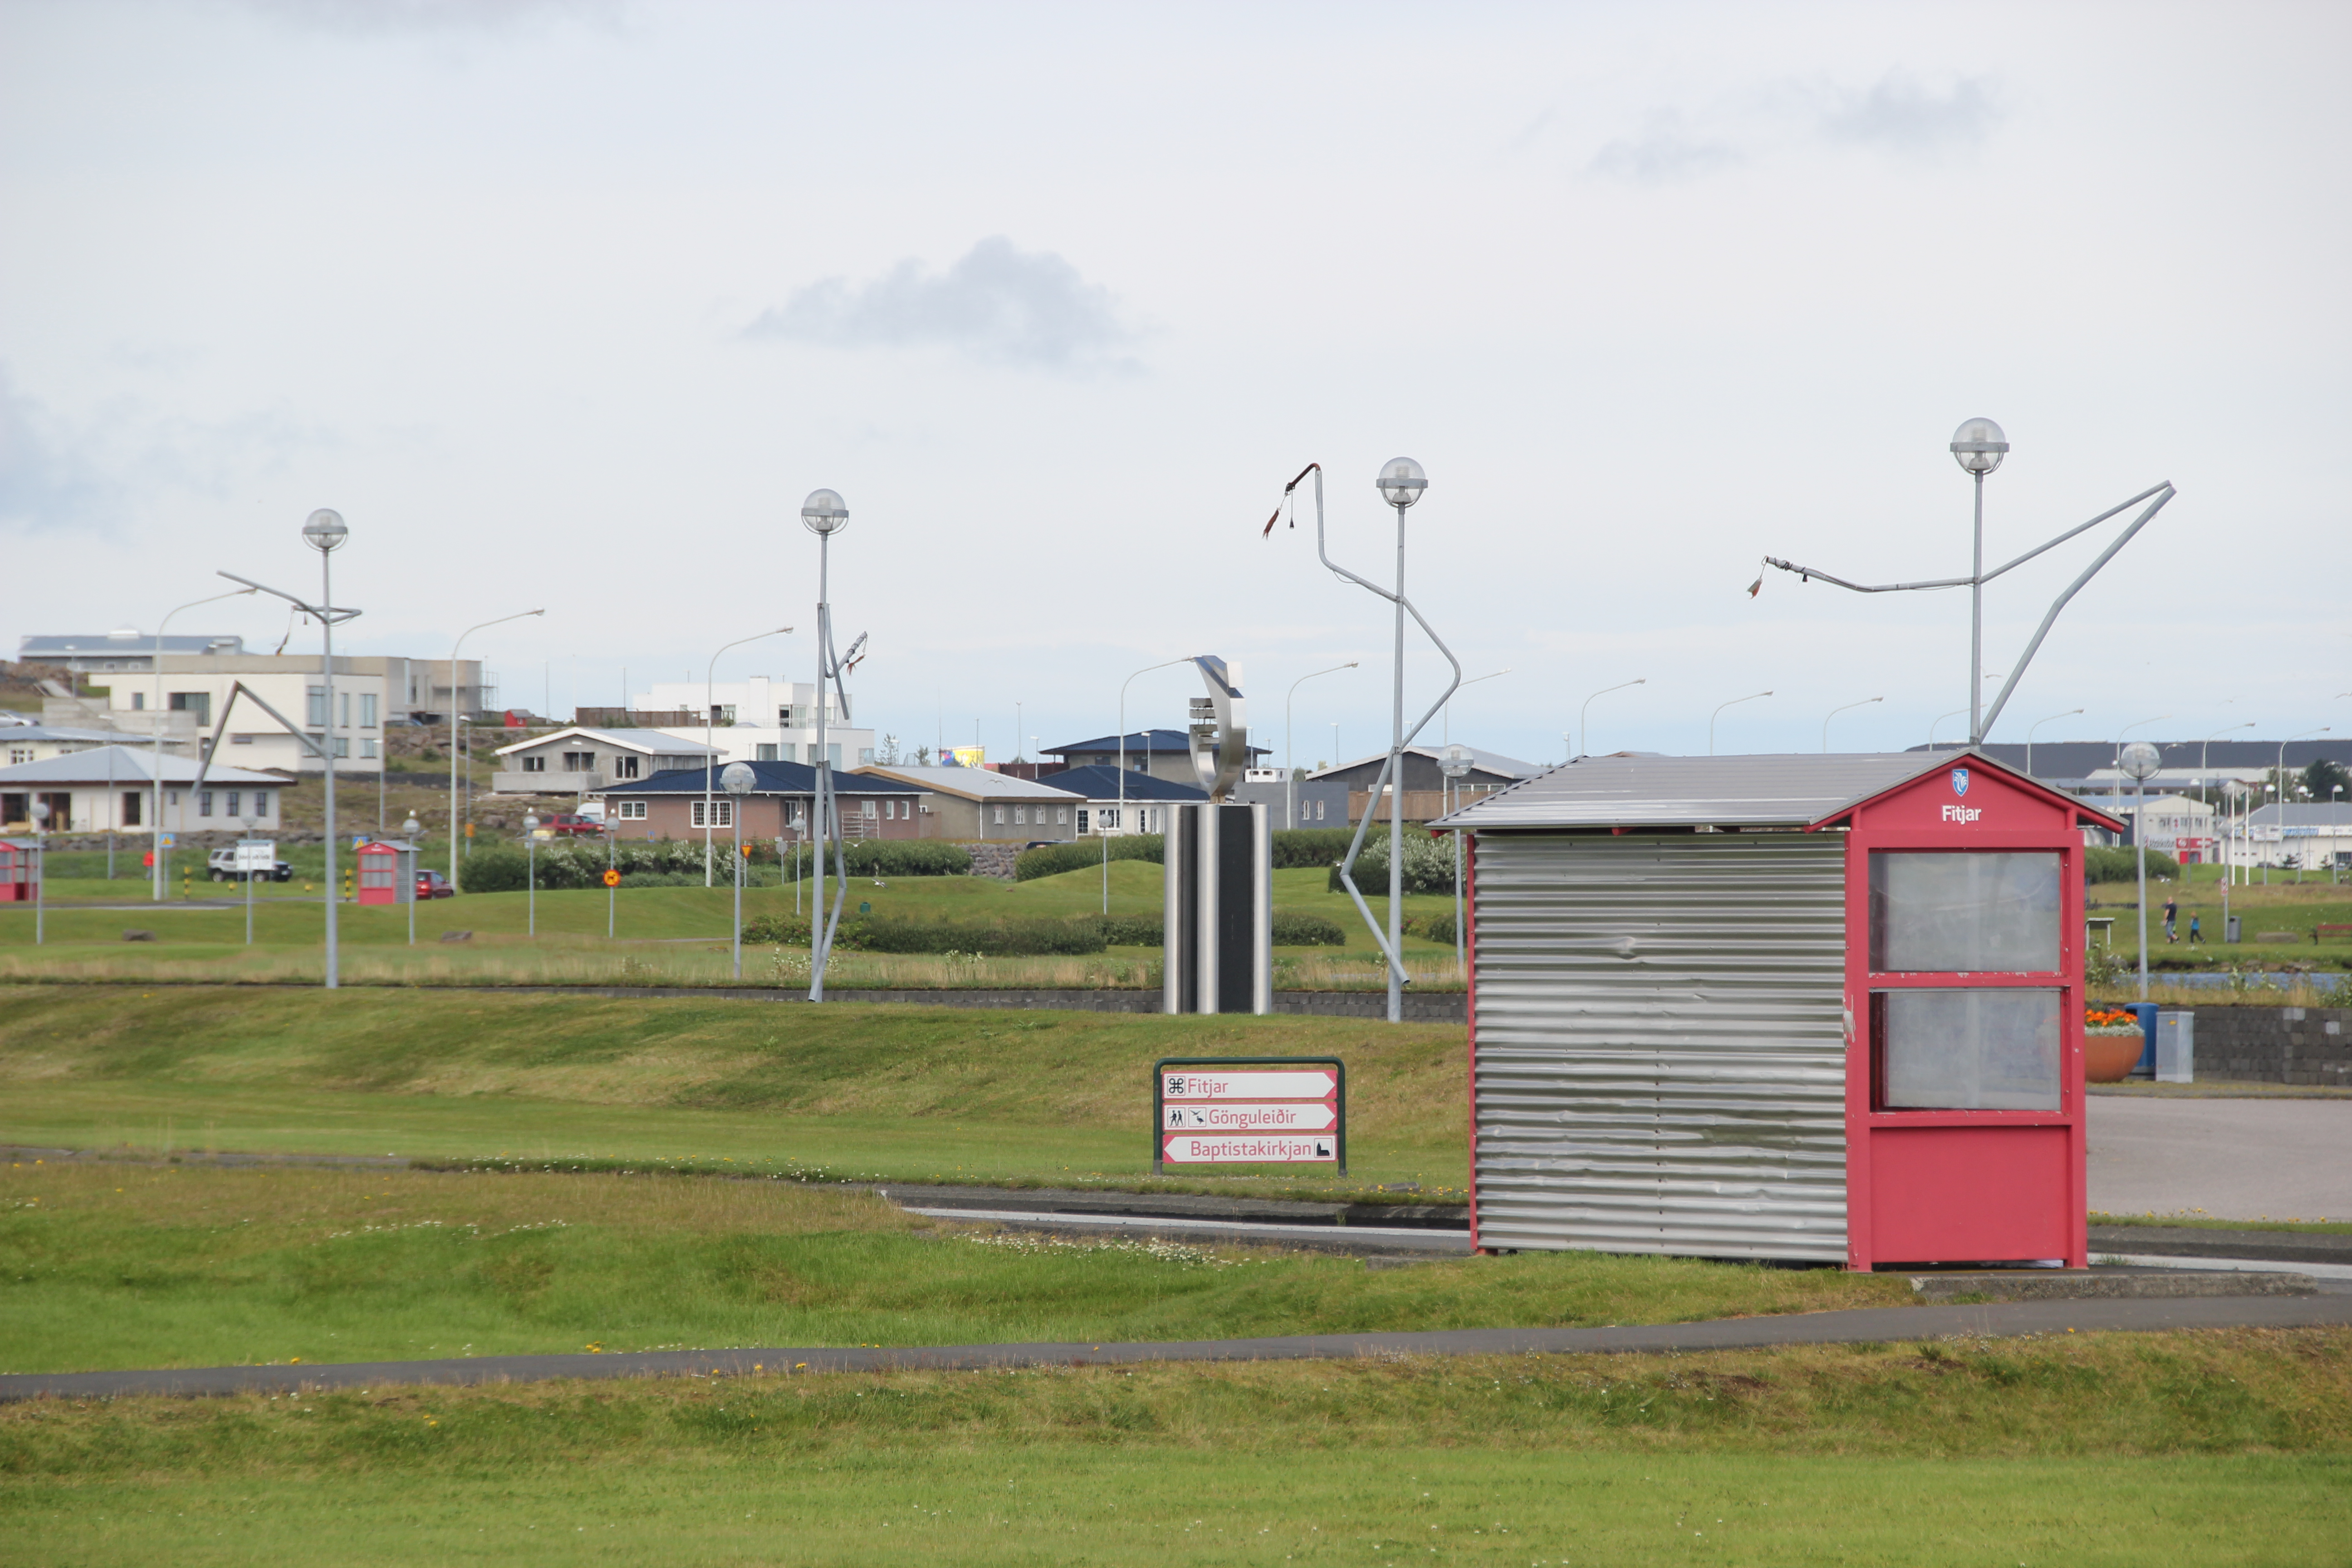
\includegraphics[width=.9\textwidth]{./photos/2014-07-22_14-53-31__2.jpg}
%  \caption{A subfigure}
%  \label{fig:keflavik_metal_guys}
%\end{subfigure}%
%\begin{subfigure}{.5\textwidth}
%  \centering
%  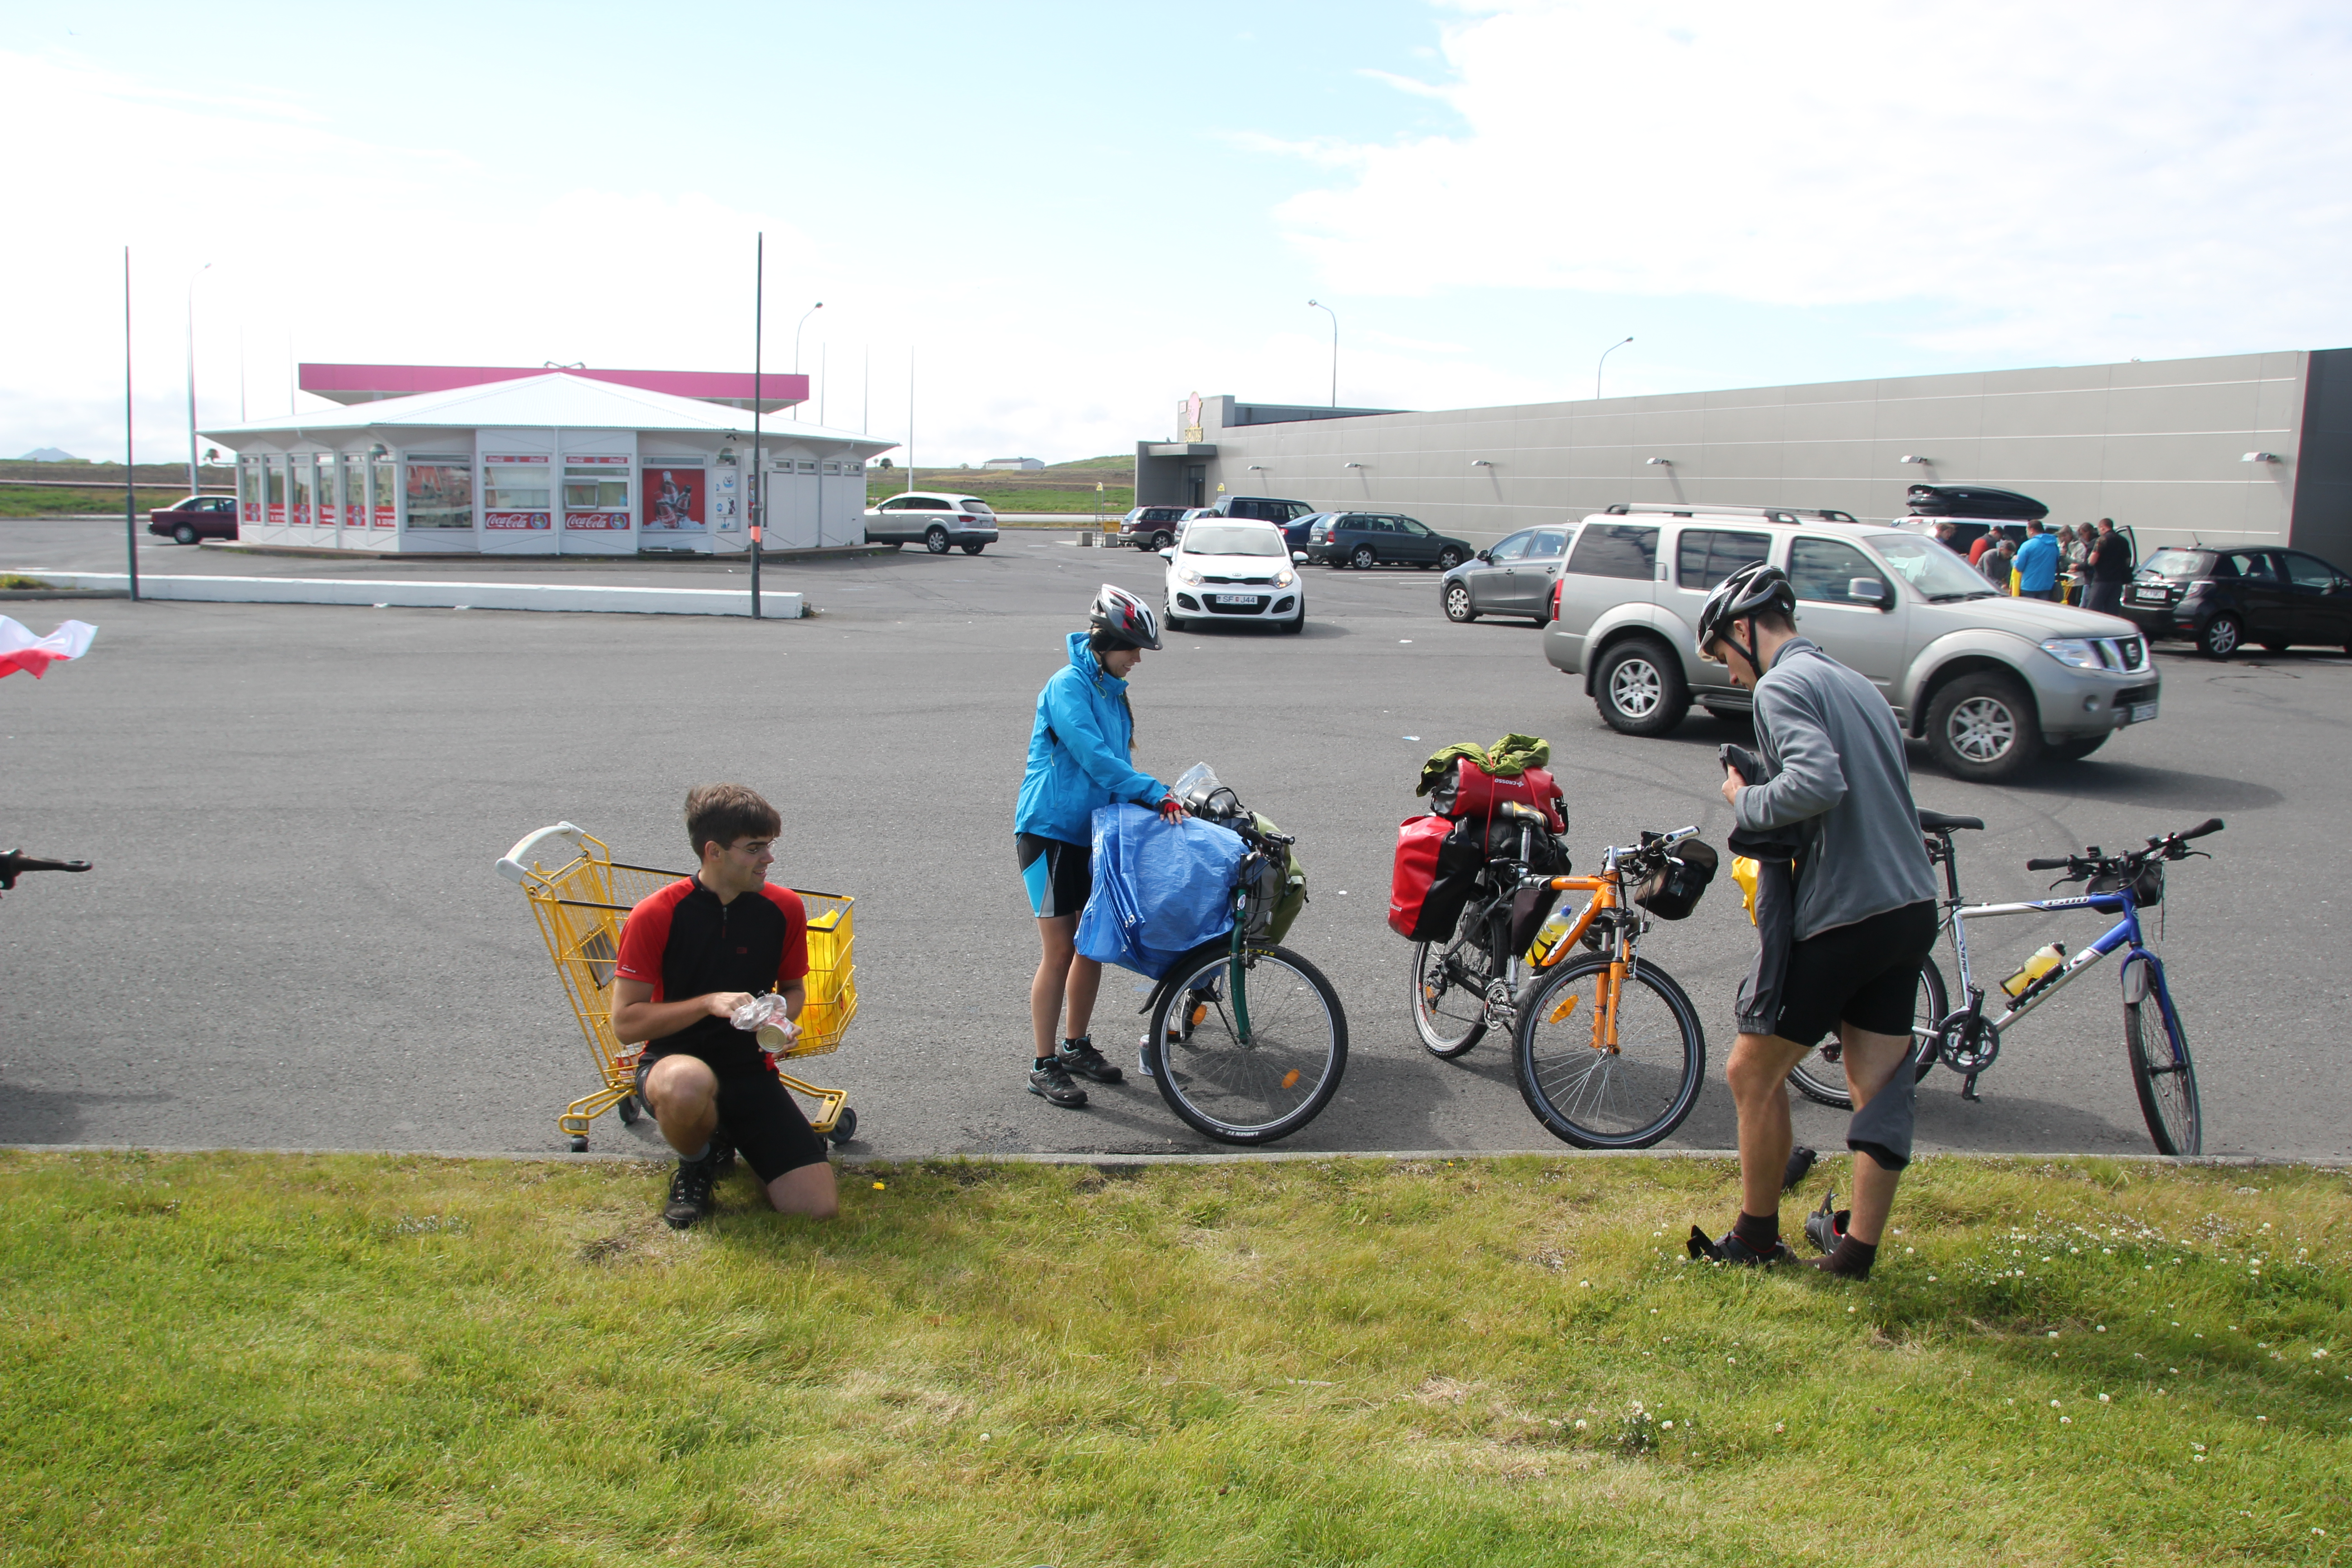
\includegraphics[width=.9\textwidth]{./photos/2014-07-22_14-54-31__3.jpg}
%  \caption{A subfigure}
%  \label{fig:keflavik_breakfast}
%\end{subfigure}
%\end{figure}

Posileni, pełni sił, ruszyliśmy do centrum Keflavíku, do oddziału Landsbanki (\href{https://www.google.com/url?q=https\%3A\%2F\%2Fmaps.google.com\%2Fmaps\%3Fq\%3D63.995522\%2C-22.548067}{mapa}) - takie PKO - by wymienić trochę waluty. Niby na lotnisku był bankomat, ale nietóre karty średnio z nim współpracowały, a do tego dziewczyny chciały wymienić trochę euro na korony…

\hint{Na Islandii naprawdę wszędzie można płacić kartą. Nawet na kempingach w środku interioru! Jedyne, co warto mieć ze sobą, to żelazną rezerwę monet o nominale 100 kr - na wielu kempingach zainstalowane są “dozowniki ciepłej wody”, które przyjmują 5x 100 kr i w zamian umożliwiają wzięcie 5-minutowego ciepłego prysznica. Czasem da się rozmienić banknoty na monety na kempingu, lecz w myśl zasady “przezorny zawsze ubezpieczony” znacznie lepiej zrobić to zawczasu w jakimś sklepie czy stacji benzynowej.}

Ostatnim puntem był zakup czegoś, co umożliwi nam dzwonienie z islandzkiego numeru komórkowego oraz korzystanie z internetu - wybór padł na Vodafone (biuro tej firmy mieściło się koło polskiego marketu), który oferował 3 GB danych za około 50 zł. O ile bez problemu kupiliśmy prepaid, o tyle aktywacja internetu wymagała już więcej zachodu, bo nie dość, że operacja odbywała się poprzez infolinię Vodafone, to jeszcze niezbędne było posiadanie karty kredytowej (szczęśliwie mieliśmy w odwodzie w Polsce posiadacza takowej). A internet miał nam służyć nie tylko do zabawy facebookiem, ale o tym później…

\hint{Zawczasu, przed wyjazdem z Polski, zorientuj się kto z rodziny / przyjaciół / znajomych posiada kartę kredytową i będzie skłonny podać ci jej numer, datę ważności oraz kod CVV. Istnieje pewna grupa usług (oprócz wspomnianej aktywacji pakietu internetowego np. zakup niektórych biletów online), których nie da się załatwić przy użyciu zwykłej karty debetowej.}

Keflavík opóściliśmy ostatecznie o 15:00, przy (wciąż jeszcze) słonecznej pogodzie.

\hint{Islandia to olbrzymi obszar i ciężko zawczasu dowiedzieć się o każdej atrakcji, każdym interesującym miejscu na trasie. Warto korzystać więc intensywnie z informacji turystycznych, zbierać (i przeglądać!) foldery reklamowe oraz pytać innych turystów (najlepiej też rowerzystów, bo ci będą w stanie np. przestrzec cię przed trudnościami terenowymi itp.). Keflavík posiada Centrum Informacji Turystycznej (\href{https://plus.google.com/111960041675886065623/about?gl=pl\&hl=en}{mapa}).}

\section*{Pierwsze godziny w trasie}

Pierwsze kilometry i już mocne zderzenie z islandzką naturą - jedziemy przez pustkowia. Po lewej, po prawej, jak okiem sięgnąć lawa i niewielkie skałki. Nic dziwnego, że obszar ten - jako jeden z trzech na Islandii - służył NASA do prowadzenia treningów dla astronautów przed misją Apollo.

\img{./photos/x-s-2014-07-22_18-05-39__5.jpg}{first_hours_on_iceland}{Pustkowia półwyspu Reykjanes}

\img{./photos/x-s-2014-07-22_18-25-14__8.jpg}{neptune_monument}{Pomnik planety Neptun}

Kawałek przed Hafnir przyplątał się do naszej grupy pies - ochrzczony Posejdonem (od \href{https://www.facebook.com/120832791270880/photos/a.612815058739315.1073741825.120832791270880/612815132072641/?type=3&theater}{pomnika planety Neptun}, który stał w miejscu zdarzenia) - który biegł za nami aż do \href{http://www.visitreykjanes.is/searchresults/attraction/bridge-between-continents}{Kładki Między Kontynentami}. Nie byłoby w tym nic aż tak specjalnego, lecz Posejdon urzekł nas swym polowaniem na samochody: gdy zauważył nadjeżdżający pojazd, zaczajał się na poboczu i potem w ostatniej chwili wypadał na jezdnię - tuż przed maskę - głośno ujadając. Albo niesamowicie odważny albo niesamowicie głupi ;-)

Już daje nam się we znaki wiatr oraz liczne (na szczęście krótkie) stromsze podjazdy. Walka z takim kombo jest szczególnie ciężka dla tych osób, które nie jeździły ostatnio za wiele.

\hint{Podczas jazdy na rowerze pracują odrobinę inne mięśnie niż np. podczas wycieczek górskich. Bieganie, pływanie, orbitrek - wszystko to oczywiście zwiększa wydolność organizmu, lecz nic nie zastąpi odpowiedniej liczby przejechanych kilometrów! :)}

Słońce było tylko na zachętę - szybko się schowało za chmury i zrobiła typowa islandzka aura - z mniej lub bardziej intensywnymi opadami deszczu… A trzeba wiedzieć, że tu nie ma się gdzie schować - żadnych przydrożnych sklepów, barów, nawet wiat PKS-u. Tak więc siłą rzeczy - mimo deszczu jedziemy dalej. Zresztą… nie lało tylko kropiło, czyli nawet nie byłoby sensu przeczekiwać tego - klimat tu bowiem taki, że możnaby się nie doczekać momentu “wypadania”.

\section*{Grindavík}

Będąc już na obrzeżach Grindavíku powstał problem - szukać miejsca na nocleg już teraz, czy może jechać jeszcze kawałek dalej? Cała ekipa była dość jednomyślna: Nie, nie jedziemy już dalej - jest za późno [była 19:00] no i warto się nie zarżnąć od razu pierwszego dnia. Lepiej wyruszyć wcześniej nazajutrz, ale przynajmniej dziś odespać podróż!” Tu konieczne jest słowo komentarza - Berlińczycy nie spali ani w Polskim Busie, ani koczując na lotnisku Schönefeld ani też w samolocie. Zatem byli non-stop na chodzie przez 30 godzin, ze względu na późny przylot i długie czekanie na bagaż noc w Ásbrú też była zarwana… Tak więc po przejechaniu 50 km rozbiliśmy się na kempingu w Grindavíku.

Kemping można zaliczyć do klasy “all inclusive”, bo posiada “świetlicę” (ogrzewanie podłogowe!) z aneksem kuchennym z pełnym wyposażeniem (sztućce, garnki, płyty indukcyjne, toster…), a prysznice są w cenie. W kuchni cała jedna szafka była zajęta przez “free stuff” - nie tylko rzeczy spożywcze, ale też gospdarcze (np. są wspomniane naboje gazowe).

\img{./photos/x-s-2014-07-23_11-11-19__6.jpg}{grindavik_cantine}{Kantyna kempingu w Grindavíku}

\hint{Warto przeglądnąć cały “free food” i “free stuff”, bo często można tam natrafić na towary luksusowe - porządną herbatę, konserwy, słodycze, płatki śniadaniowe… Należy jednak zwracać uwagę na termin przydatności do spożycia oraz organoleptycznie zbadać faktyczny stan produktu (np. otwartego mleka lepiej nie tykać ;-)}

Na obiadokolację z radością pochłaniamy spaghetti z mięsem ze słoika (polskie, domowe, zawekowane mięso - mniam!), sosem i warzywami z puszki. Przekąszamy ciasteczkami i niezwłocznie udajemy się na spoczynek - większość z nas nawet bez mycia się…

\hint{Kupując warzywa i sosy w puszcze warto zwrócić uwagę na “gęstość” produktu, tj. stosunek wagi netto (po odcieku) do wagi brutto - bo po co wozić ze sobą puszkowaną wodę?! Na Islandii bezkonkurencyjna pod tym względem okazała się mieszanka warzyw Euroshopper, w której wspomniany współczynnik wynosił około 0,95.}

Karolina: Czuję się, jakbym była na Islandii od tygodnia…
Ponieważ mamy intrnet i założone wydarzenie na fb (co by nie musieć powtarzać po parę razy tego samego - gdzie jesteśmy i co robimy - i rodzinie i znajomym), więc co jakiś czas Put informuje nas, że “O! Mamy 5 lajków i 3 komentarze!”. Hm.. może należało założyć profil fb? Wtedy moglibyśmy jeszcze korzystać ze statystyk…
Internet wprowadza też nową jakość wieczorami, przed spaniem. W pewnym momencie rozlega się dramatyczne wołanie: “Pucie, zrobisz modem?”, a chwilę później: “Pucie, przełożysz komórkę bliżej naszego namiotu? Bo coś słaby zasięg…”
